\documentclass[12pt,a4paper]{article}

\usepackage{graphicx}% Include figure files
\usepackage{dcolumn}% Align table columns on decimal point
\usepackage{bm}% bold math
%\usepackage{hyperref}% add hypertext capabilities
%\usepackage[mathlines]{lineno}% Enable numbering of text and display math
%\linenumbers\relax % Commence numbering lines

%\usepackage[showframe,%Uncomment any one of the following lines to test 
%%scale=0.7, marginratio={1:1, 2:3}, ignoreall,% default settings
%%text={7in,10in},centering,
%%margin=1.5in,
%%total={6.5in,8.75in}, top=1.2in, left=0.9in, includefoot,
%%height=10in,a5paper,hmargin={3cm,0.8in},
%]{geometry}

\usepackage{multicol}%Para hacer varias columnas
\usepackage{multicol,caption}
\usepackage{multirow}

\setlength{\topmargin}{-1.0in}
\setlength{\oddsidemargin}{-0.3pc}
\setlength{\evensidemargin}{-0.3pc}
\setlength{\textwidth}{6.75in}
\setlength{\textheight}{9.5in}
\setlength{\parskip}{0.5pc}

\usepackage[utf8]{inputenc}
\usepackage{expl3,xparse,xcoffins,titling,kantlipsum}
\usepackage{graphicx}
\usepackage{xcolor} 
\usepackage{nopageno}
\usepackage{lettrine}
\usepackage{caption}
\captionsetup[table]{name=Tabla}
\renewcommand{\figurename}{Figura}
\usepackage{float}
\renewcommand\refname{Bibliograf\'ia}
\usepackage{amssymb}
\usepackage{amsmath}
\usepackage[rightcaption]{sidecap}
\usepackage[spanish]{babel}

% CABECERA Y PIE DE PÁGINA %%%%%
\usepackage{fancyhdr}
\pagestyle{fancy}
\fancyhf{}

\begin{document}
\noindent \textbf{a) Entra a \underline{stokes.fciencias.unam.mx} con el usuario grupo2021 y contraseña alumnox2021 y en el directorio hogar crea un directorio con tu nombre y primer apellido por ejemplo:
edgar\_vazquez (usa guión bajo y sólo minúsculas).}

\noindent Para entrar a stokes se puede usar ssh con la opción -l y con el usuario grupo2021 como se ve en la figura 1.

\begin{figure}[h!]
    \centering
    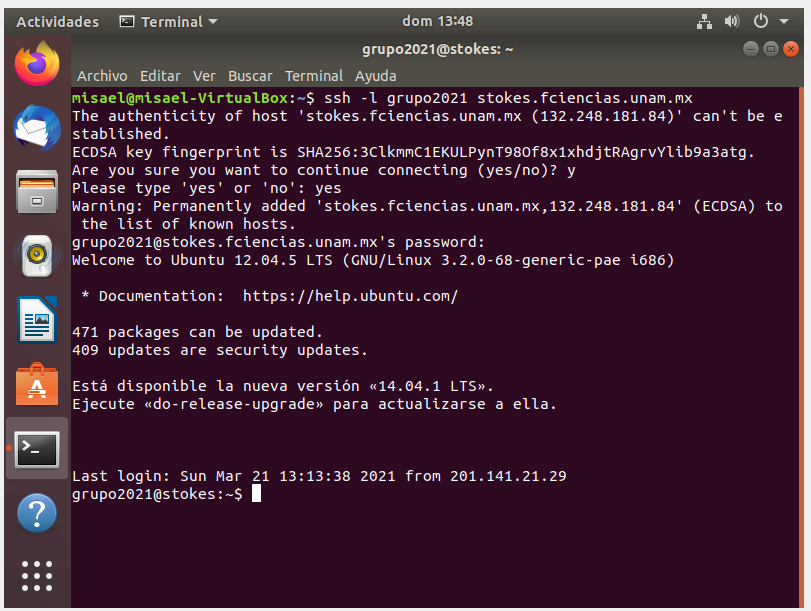
\includegraphics[scale = 0.5]{a.1.png}
    \caption{}
\end{figure}

\noindent En la figura 2 se muestra como usar el comando mkdir sin opciones para crear un directorio en la dirección de trabajo, se puede confirmar su creación con el comando ls.
\begin{figure}[h!]
    \centering
    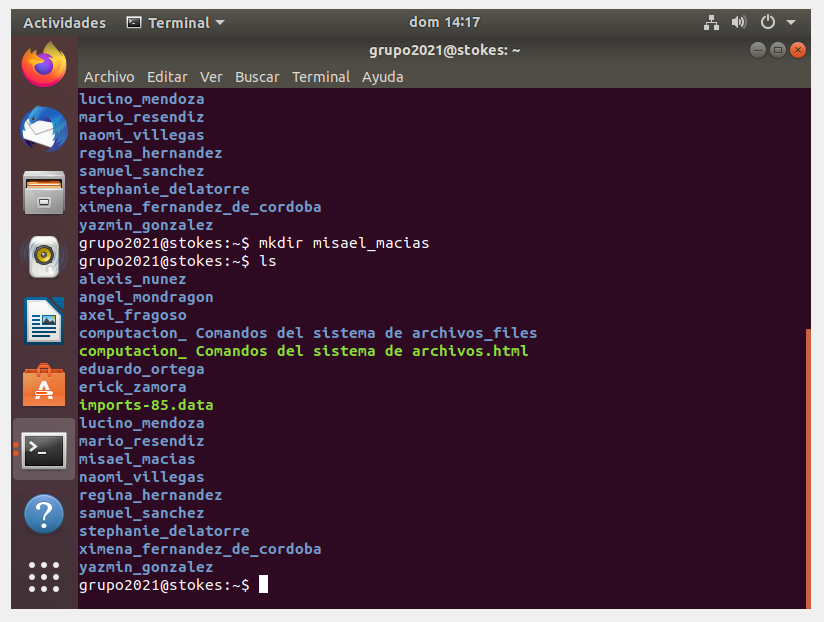
\includegraphics[scale = 0.5]{a.2.png}
    \caption{}
\end{figure}
\newpage

\noindent \textbf{b) Crea el siguiente ambiente de trabajo a partir del directorio con tu nombre:}


\begin{figure}[h!]
    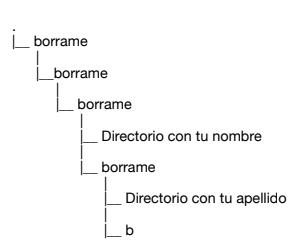
\includegraphics[scale = 0.9]{b.dir.png}
\end{figure}

\noindent En la figura 3 se puede una manera distinta a el inciso a) para crear directorios que es ideal para crear muchos directorios, esto se hace con mkdir y con la opción -p, también se puede ver una forma de visualizar el árbol creado anteriormente con el comando tree.

\begin{figure}[h!]
    \centering
    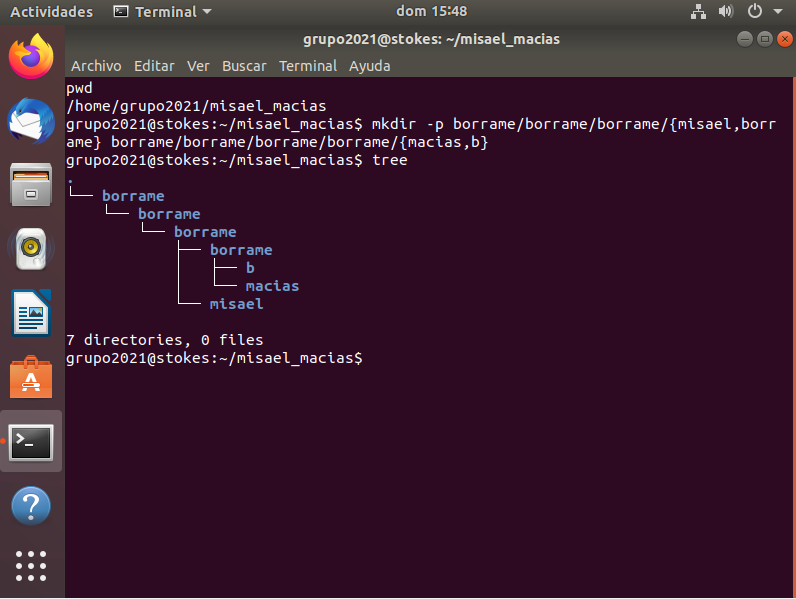
\includegraphics[scale = 0.5]{b.1.png}
    \caption{}
\end{figure}
\\
\newpage

\noindent \textbf{c) En el directorio b crea un archivo nombre.txt que contenga tu nombre}

\noindent En la figura 4 se usa el comando cat para crear un archivo de texto de forma primitiva y que nos permite modificar al momento de ser creado, también se muestra como moverse entre directorios usando el comando cd con su respectiva ruta.
\begin{figure}[h!]
    \centering
    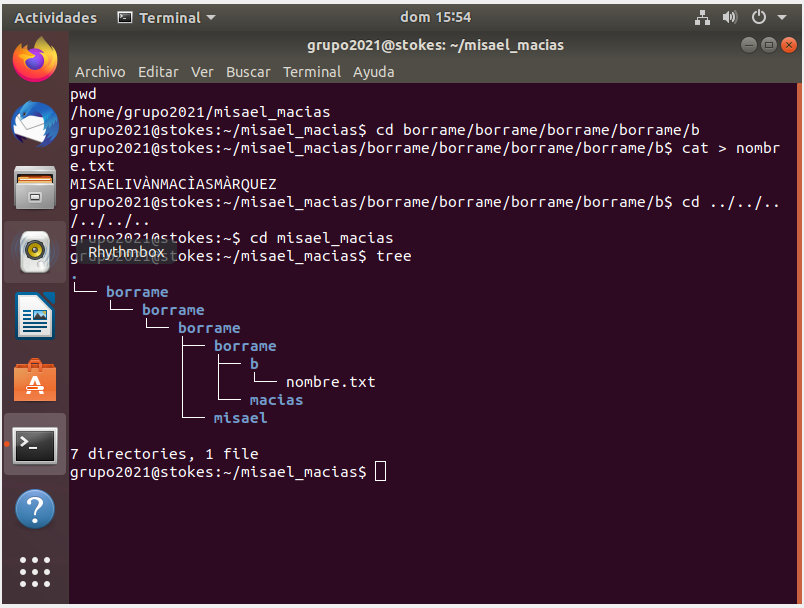
\includegraphics[scale = 0.5]{c.1.png}
    \caption{}
\end{figure}


\noindent \textbf{d) Mueve el archivo nombre.txt para que este junto al primer borrame es decir inmediatamente
en el primer subdirectorio abajo de tu nombre}

\noindent En la figura 5 se utiliza el comando mv con la opción -f para mover un archivo, pero primero se mueve el directorio de trabajo al directorio que contiene dicho archivo
\begin{figure}[h!]
    \centering
    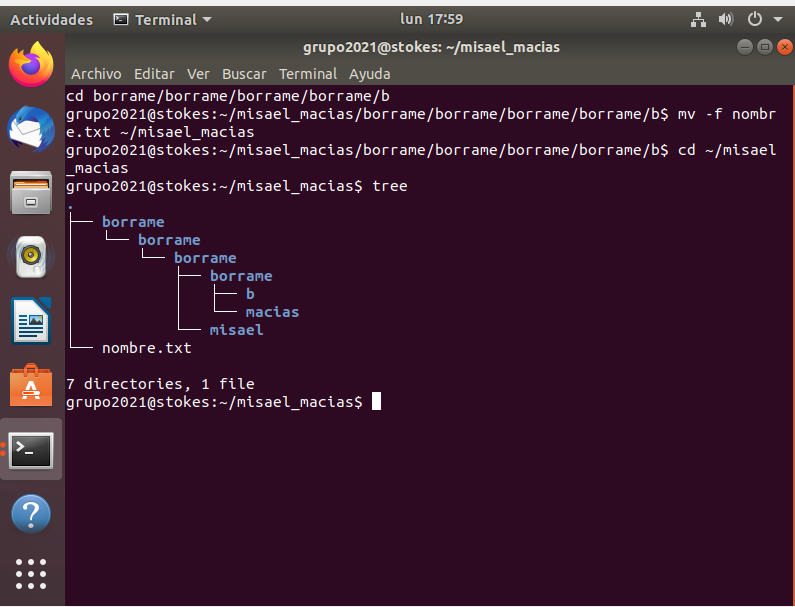
\includegraphics[scale = 0.5]{d.1.png}
    \caption{}
\end{figure}

\noindent \textbf{e) Copia a tu computadora local los siguientes archivos que se encuentran en stokes:}

\noindent \textbf{e.1)Primero entra a stokes y cerciórate que efectivamente están ahí, explica cómo haces
esto, explicar todo (comados).}

\noindent \textbf{computacion\_ Comandos del sistema de archivos\_files (este es un directorio recuerda usar -r) computacion\_ Comandos del sistema de archivos.html imports-85.data}


\noindent \textbf{\emph{Nota importante}: Cómo desgraciadamente los nombres (dos de los archivos) tienen espacios en blancos, esto es un problema en linux porque el espacio significa separar archivos, así que
tendríamos que “escapar” el significado esto se logra con \ (diagonal invertida) pero para que
sea más fácil mejor utilizaremos el asterisco (*) que significa cero o mas caracteres así si
ponemos computacion* en el comando cp significará que se traiga los dos primeros archivos
de un jalón (recuerda el -r)}

\noindent En la figura 6 se usa el comando scp con la opción -r, para los archivos con espacio en el nombre se usa un * para descargar todos los archivos en la carpeta hogar que empiezan con los caracteres anteriores al asterisco
\begin{figure}[h!]
    \centering
    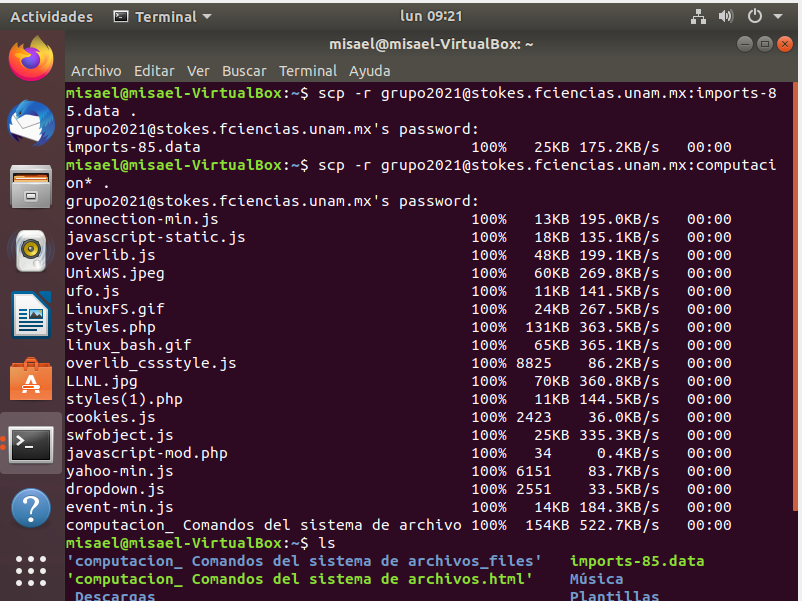
\includegraphics[scale = 0.5]{e.1.png}
    \caption{}
\end{figure}
\\
\newpage

\noindent \textbf{f) En stokes entra al directorio /dev y localiza 5 archivos tipo carácter (recuerda lo que vimos en clase sino ve el video) como los copiarías al directorio (utiliza \{\}) con tu nombre con ruta absoluta y relativa ¡NO LO HAGAS! por favor solo di cómo hacerlo. Localiza 5 tipo “bloque” y di como los copiarías al directorio b de nuevo ¡NO LO HAGAS!.}

\noindent Primero para moverse a dev se puede usar cd partiendo desde la raíz dado que dev es un subdirectorio de la misma, después para encontrar los archivos tipo carácter en el directorio dev se usa el comando find  con la dirección /dev y con - type c para buscar tipo carácter, también se usa la opción -exec y el comando cp con la dirección a donde se va a copiar (../home/grupo2021/misael\_macias, como relativa y /home/grupo2021/misael\_macias como absoluta) y se termina con {} \;

\noindent para los archivos tipo bloque se puede usar el mismo comando pero con - type b y con la misma opción -exec y comando cp pero con distinta ruta 

\noindent (../home/grupo2021/misael\_macias/borrame/borrame/borrame/borrame/b como relativa y 

/home/grupo2021/misael\_macias/borrame/borrame/borrame/borrame/b como absoluta) 

\end{document}
